% !TEX root = ../report.tex
\section{Das Graphical User Interface}
\begin{Spacing}{\mylinespace}

Zur Interaktion und Einstellung der einzelnen Komponenten entschieden wir uns dafür, unserer Anwendung ein \textit{Graphical User Interface} (GUI) zu spendieren. 

\subsection{Die Anforderungen}

Als Anforderungen setzten wir uns ein übersichtliches und leicht verständliches System, welches uns im Laufe des Projekts ermöglichen sollte, schnell und ohne größeren Aufwand, neue Funktionalitäten hinzuzufügen.  

\subsection{Die Umsetzung}

Um diese Anforderungen zu erreichen experimentierten wir im ersten Projektsemester mit einem \textit{Multi-Window} Ansatz auf Basis von \textit{Windows Forms}. Dieser Ansatz bestand aus zwei separaten Fenstern (s. Abbildung \ref{fig:GUIOld}). Ein Fenster, das für die Projektion auf den Sand, mit Hilfe des Beamers genutzt wurde und ein weiteres Fenster für die 3D-Ansicht, Zusatzinformationen und den Bedienelementen zur Anpassung des Systems.
\\\\
Leider stellte sich recht schnell heraus, dass dieser Ansatz doch nicht ganz so flexibel war, wie anfangs erwartet und das hinzufügen von neuen Bedienelementen jedes Mal mit relative viel Arbeit verbunden war. Zudem bedeuteten die beiden Fenster auch die doppelte Arbeit, da die komplette Szene jeweils zweimal gezeichnet werden musste. Aus diesen Gründen, entschlossen wir uns zu Beginn des zweiten Projektsemesters, diesen Ansatz zu verwerfen und auf ein einzelnes Fenster mit einer GPU-basierten GUI zu setzen.

\begin{figure}[h!]
	\centering
	\vspace*{30px}
	\includegraphics[width=320px]{graphics/gui.png}	
	\caption{Multi-Window GUI aus dem ersten Projektsemester.}
	\label{fig:GUIOld}
\end{figure}

\begin{description}
	\item[Ruminate GUI] \hfill \\
	Nach längerer Recherche und Suche nach einer passenden Bibliothek zur Darstellung eines GUI unter XNA, entschieden wir uns letztendlich für die sehr minimalistische, Open-Source Bibliothek \textit{Ruminate} \cite{Fra13}. Diese bot uns grundlegende Bedienelemente (s. Abbildung \ref{fig:Ruminate}) wie Buttons, Slider, usw. und war weitaus weniger überladen als die meisten anderen Bibliotheken.
\\\\
Natürlich hatte auch diese Bibliothek nicht nur Vorteile. Da diese von einem Ein-Mann-Team als Hobbyprojekt entwickelt wurde, gab es hier und da noch das ein oder andere Problem und auch das Design der Bedienelemente war nicht das schönste. Dank Open-Source, konnten wir uns aber selbst um diese Probleme kümmern und das GUI individuell an unser System anpassen.
	
\begin{figure}[h!]
	\centering
	\vspace*{20px}
	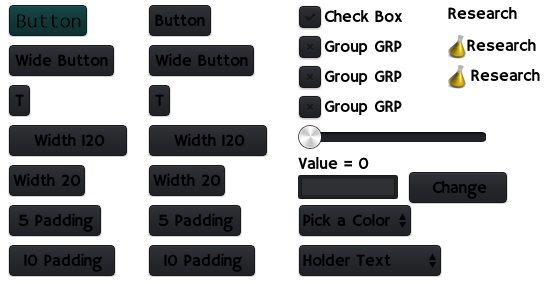
\includegraphics[width=280px]{graphics/ruminate.png}	
	\caption{Einige Bedienelemente der Ruminate GUI \cite{Fra13}.}
	\label{fig:Ruminate}
\end{figure}
	
	\item[Reflections] \hfill \\
	
	
\begin{figure}[h!]
	\vspace*{30px}
	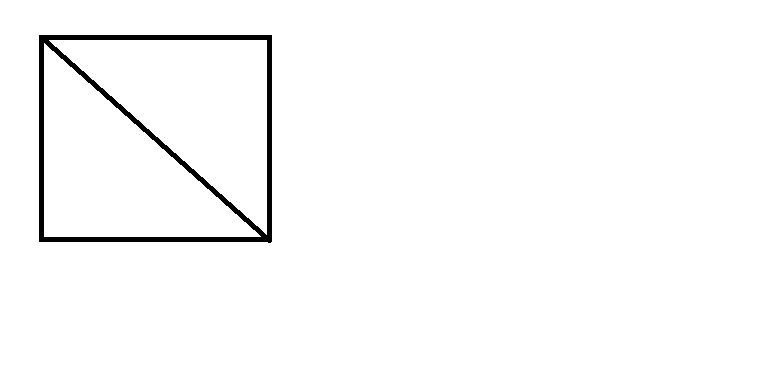
\includegraphics[width=\columnwidth]{graphics/reflection.png}	
	\caption{Reflection}
	\label{fig:Reflection}
\end{figure}
	
\end{description}

\subsection{Das Ergebnis}

\begin{figure}[h!]
	\centering
	\vspace*{30px}
	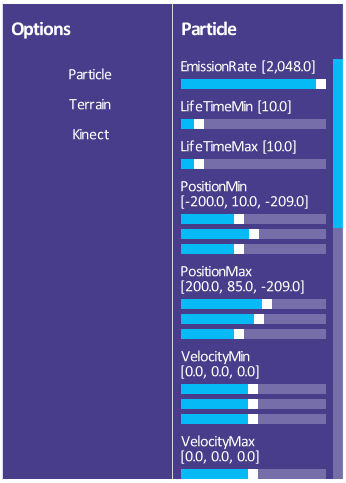
\includegraphics[width=210px]{graphics/newGui.png}
	\caption{Die ingame GUI.}
	\label{fig:NewGUI}
\end{figure}

\begin{figure}[h!]
	\centering
	\vspace*{30px}
	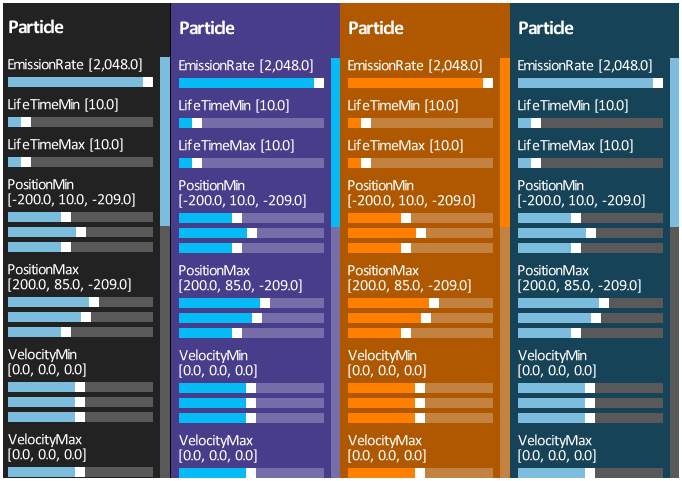
\includegraphics[width=\columnwidth]{graphics/guiThemes.png}
	\caption{Unterschiedliche Erscheinungsbilder der GUI.}
	\label{fig:GUIThemes}
\end{figure}

\end{Spacing}
\newpage

\section{Reflection}
Im Laufe der Zeit wurde unser Projekt immer größer, dies brachte auch viele neue Funktionalitäten mit sich.
All diese neuen Features mussten wir stetig unserer GUI-Oberfläche hinzufügen. Dieser sehr statische Ansatz wurde deshalb durch Reflektion in einen dynamischen überführt.
Diverse moderne Programmiersprachen so auch unser verwendetes C-Sharp besitzen die Möglichkeit während des Programmablaufs Informationen über die Struktur eines gegebenen Objekts abzurufen.



Dieser Ansatz und die Tatsache das wir diverse Probleme mit unserer statischen Multi-Window GUI hatten, haben uns dazu bewegt unser altes GUI-System abzulösen.
Dank unseren Properties war es uns mittels Reflection möglich ein neues dynamisches GUI System einzuführen, hierbei verzichteten wir auch auf das Multi-Window System und haben die GUI direkt auf den Sandkasten projeziert.


\clearpage
%% End Of Doc